\setcounter{page}{2}
\section*{Цель работы}
Разработать программу, реализующую представление определенного набора примитивов из имеющихся в библиотеке OpenGL (GL\_POINT, GL\_LINES, GL\_LINE\_STRIP, GL\_LINE\_LOOP, GL\_TRIANGLES, GL\_TRIANGLE\_STRIP, GL\_TRIANGLE\_FAN, GL\_QUADS, GL\_QUAD\_STRIP, GL\_POLYGON).

Разработанная на базе шаблона программа должна быть пополнена возможностями остановки интерактивно различных атрибутов примитивов рисования через вызов соответствующих элементов интерфейса пользователя.

\section*{Основные теоретические положения}
В данной лабораторной работе должны быть рассмотрены следующие примитивы:

GL\_POINTS – каждая вершина рассматривается как отдельная точка, параметры которой не зависят от параметров остальных заданных точек.
При этом вершина n определяет точку n.
Рисуется N точек (n – номер текущей вершины, N – общее число вершин).

Основой графики OpenGL являются вершины.
Для их определения используется команда glVertex.

void glVertex[2 3 4][s i f d](type coord)

Вызов команды определяется четырьмя координатами x, y, z и w.
При этом вызов glVertex2* устанавливает координаты x и y, координата z полагается равной 0, а w – 1.
Вызов glVertex3* устанавливает координаты x, y, z, а w равно 1.

GL\_LINES – каждая пара вершин рассматривается как независимый отрезок.
Первые две вершины определяют первый отрезок, следующие две – второй отрезок и т.д., вершины (2n-1) и 2n определяют отрезок n.
Всего рисуется N/2 линий.
Если число вершин нечетно, то последняя просто игнорируется.

GL\_LINE\_STRIP – в этом режиме рисуется последовательность из одного или нескольких связанных отрезков.
Первая вершина задает начало первого отрезка, а вторая – конец первого, который является также началом второго.
В общем случае, вершина n (n > 1) определяет начало отрезка n и конец отрезка (n - 1).
Всего рисуется (N - 1) отрезок.

GL\_LINE\_LOOP – осуществляется рисование замкнутой кривой линии.
Первая вершина задает начало первого отрезка, а вторая – конец первого, который является также началом второго.
В общем случае, вершина n (n > 1) определяет начало отрезка n и конец отрезка (n - 1).
Первая вершина является концом последнего отрезка. Всего рисуется N отрезков.

GL\_TRIANGLES – каждая тройка вершин рассматривается как независимый треугольник.
Вершины (3n-2), (3n-1), 3n (в таком порядке) определяют треугольник n.
Если число вершин не кратно 3, то оставшиеся ( одна или две) вершины игнорируются.
Всего рисуется N/3 треугольника.

GL\_TRIANGLE\_STRIP - в этом режиме рисуется группа связанных треугольников, имеющих общую грань.
Первые три вершины определяют первый треугольник, вторая, третья и четвертая – второй и т.д. для нечетного n вершины n, (n+1) и (n+2) определяют треугольник n.
Для четного n треугольник определяют вершины (n+1), n и (n+2).
Всего рисуется (N-2) треугольника.

GL\_TRIANGLE\_FAN - в этом режиме рисуется группа связанных треугольников, имеющих общие грани и одну общую вершину.
Первые три вершины определяют первый треугольник, первая, третья и четвертая – второй и т.д. Всего рисуется (N-2) треугольника.

GL\_QUADS – каждая группа из четырех вершин рассматривается как независимый четырехугольник.
Вершины (4n-3), (4n-2), (4n-1) и 4n определяют четырехугольник n.
Если число вершин не кратно 4, то оставшиеся (одна, две или три) вершины игнорируются.
Всего рисуется N/4 четырехугольника.

GL\_QUAD\_STRIP – рисуется группа четырехугольников, имеющих общую грань.
Первая группа из четырех вершин задает первый четырехугольник.
Третья, четвертая, пятая и шестая задают второй четырехугольник.

GL\_POLYGON – задет многоугольник.
При этом число вершин равно числу вершин рисуемого многоугольника.

\begin{figure}[h]
    \center{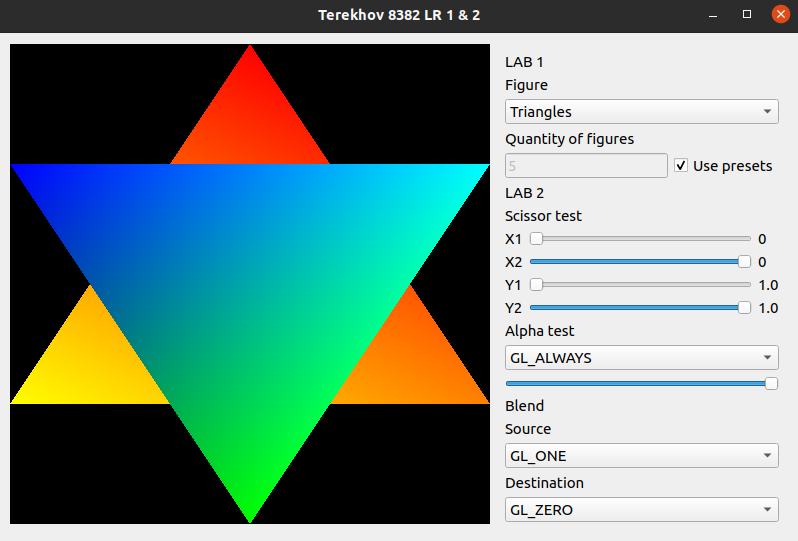
\includegraphics[scale=0.7]{1}}
    \caption{Примитивы}
    \label{fig:1}
\end{figure}

\section*{Ход работы}
Для выполнения работы был выбран язык Python 3.8 с библиотеками PyQt5 и PyOpenGL.
Для их установки необходимо воспользоваться командами:\\
\texttt{pip install pyqt5 PyOpenGL PyOpenGL\_accelerate}

Запуск программы:\\
\texttt{python3 main.py}

В коде программы библиотеки подключены таким образом:\\
\texttt{
    from PyQt5 import QtCore, QtWidgets \\
    from OpenGL.GL import * \\
    from PyQt5.QtOpenGL import QGLWidget
}

Для отображения примитивов был переопределен метод класса \texttt{QGLWidget paintGL()}:

\small{
    \begin{verbatim}
    def paintGL(self):
        glClearColor(0, 0, 0, 0)
        glClear(GL_COLOR_BUFFER_BIT | GL_DEPTH_BUFFER_BIT)
        glEnable(GL_SCISSOR_TEST)
        glEnable(GL_ALPHA_TEST)
        glEnable(GL_BLEND)
        glAlphaFunc(ALPHA[self.cur_alpha], self.alpha_value)
        glBlendFunc(BLEND_SRC[self.blend_src], BLEND_DEST[self.blend_dest])
        glScissor(self.x_clip, self.y_clip, self.w_clip, self.h_clip)
        self.show_figure()
        glDisable(GL_BLEND)
        glDisable(GL_ALPHA_TEST)
        glDisable(GL_SCISSOR_TEST)
    \end{verbatim}}
\normalsize Вспомогательный метод \verb show_figure()  занимается размещением вершин и их окраской:

\small{
    \begin{verbatim}
        def show_figure(self):
            self.cur_color_index = 0
            glBegin(self.cur_figure)
            for point in self.points:
                glColor4f(*self.get_color())
                glVertex2d(point[0], point[1])
                if len(point) >= 4:
                    glColor4f(*self.get_color())
                    glVertex2d(point[2], point[3])
                if len(point) >= 6:
                    glColor4f(*self.get_color())
                    glVertex2d(point[4], point[5])
                if len(point) >= 8:
                    glColor4f(*self.get_color())
                    glVertex2d(point[6], point[7])
            glEnd()
    \end{verbatim}}
\normalsize Данный метод принимает список списков координат точек.
Каждый вложенный список отвечает за отображение одной фигуры.

Интерфейс программы представлен на рисунке 2.
\begin{figure}[H]
    \centering
    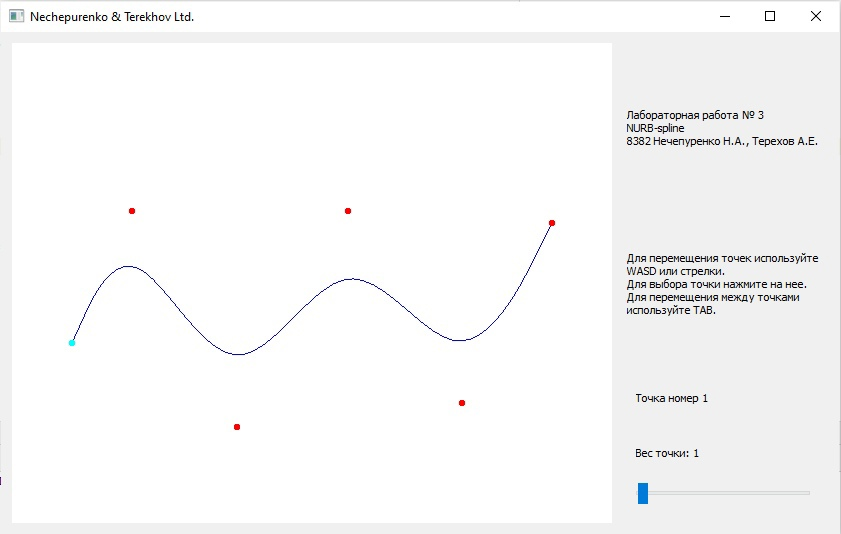
\includegraphics[width=10cm]{2}
    \caption{Интерфейс}
    \label{fig:2}
\end{figure}

Окно можно разбить на две части: левая -- область отображения, правая -- область навигации.
В области навигации можно выбрать какие примитивы нужно отобразить, указать количество фигур и установить флаг -- отображать предустановленную конфигурацию точек или устанавливать точки случайным образом.
При изменении каких-либо параметров рисунок будет изменяться.
Цвета перебираются циклично в соответствии с радугой.

Примеры работы программы представлены на рисунках 3-12.
\begin{figure}[H]
    \centering
    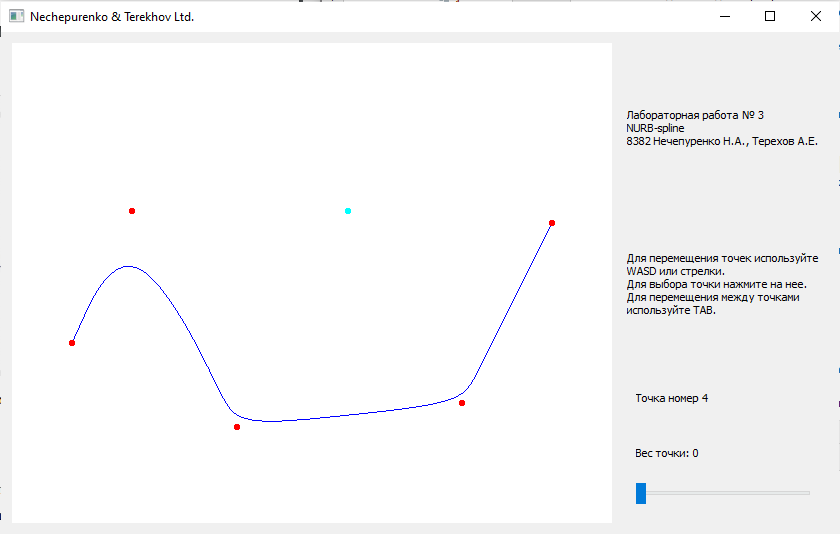
\includegraphics[width=10cm]{3}
    \caption{Примитив GL\_POINTS}
    \label{fig:3}
\end{figure}
\begin{figure}[H]
    \centering
    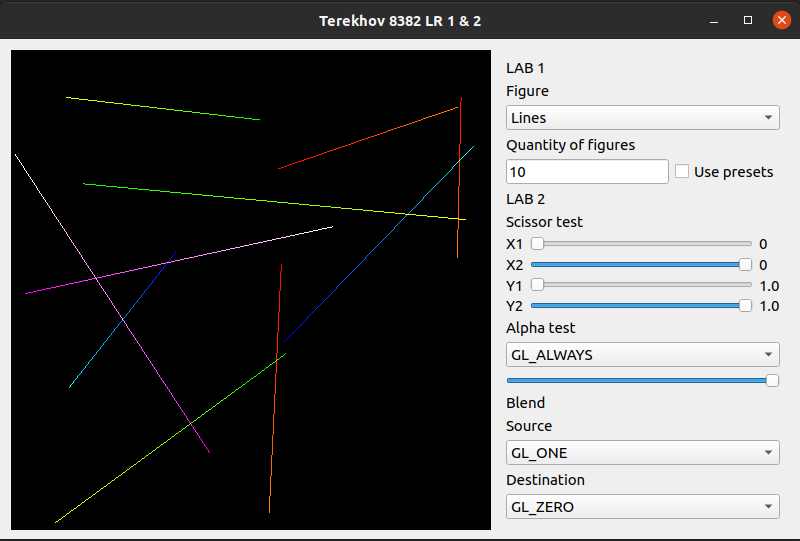
\includegraphics[width=10cm]{4}
    \caption{Примитив GL\_LINES}
    \label{fig:4}
\end{figure}
\begin{figure}[H]
    \centering
    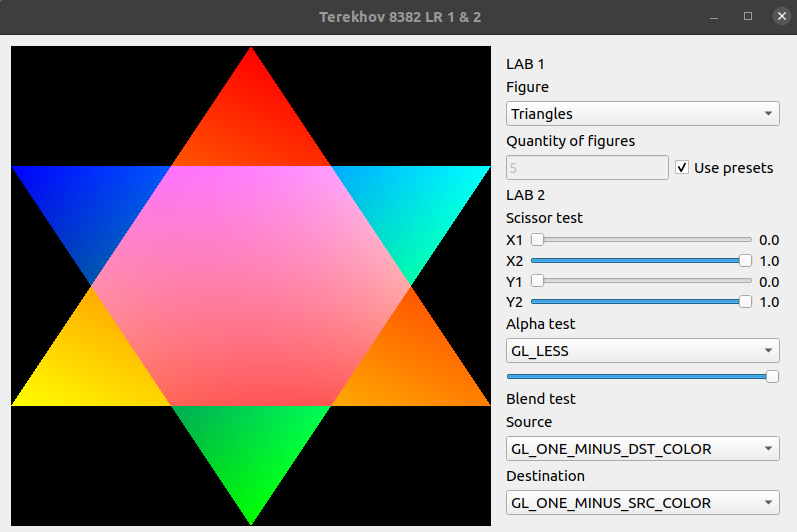
\includegraphics[width=10cm]{5}
    \caption{Примитив GL\_LINE\_STRIP}
    \label{fig:5}
\end{figure}
\begin{figure}[H]
    \centering
    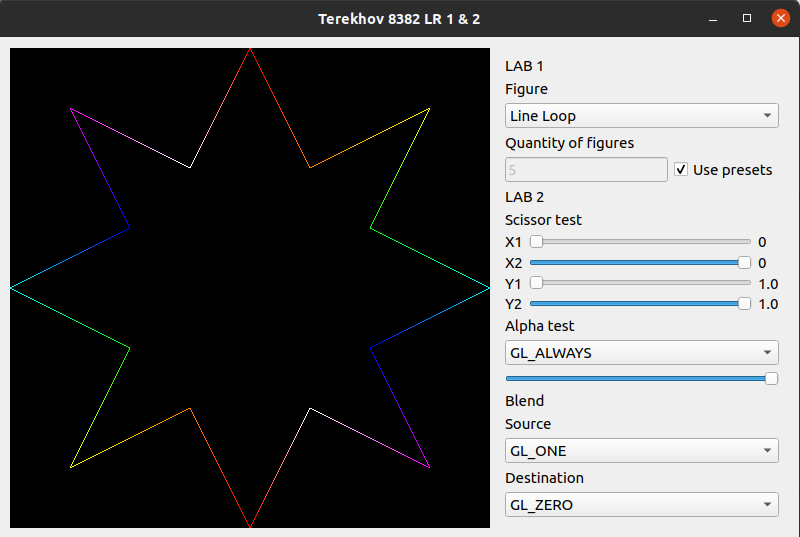
\includegraphics[width=10cm]{6}
    \caption{Примитив GL\_LINE\_LOOP}
    \label{fig:6}
\end{figure}
\begin{figure}[H]
    \centering
    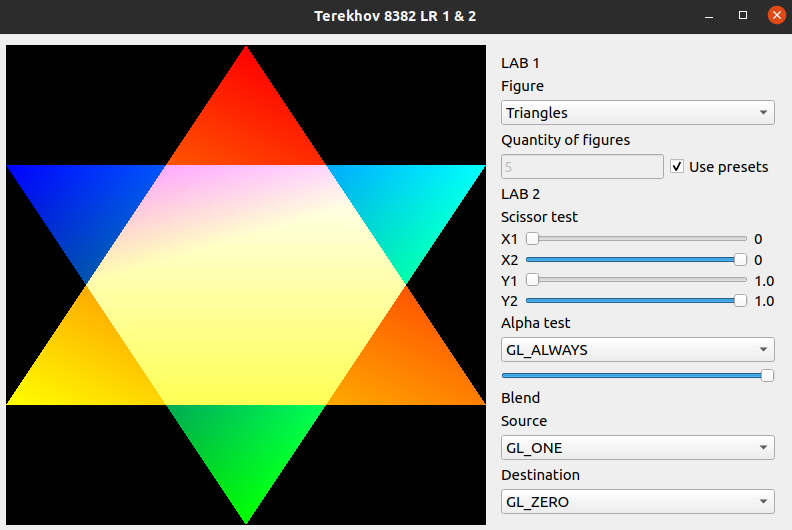
\includegraphics[width=10cm]{7}
    \caption{Примитив GL\_TRIANGLES}
    \label{fig:7}
\end{figure}
\begin{figure}[H]
    \centering
    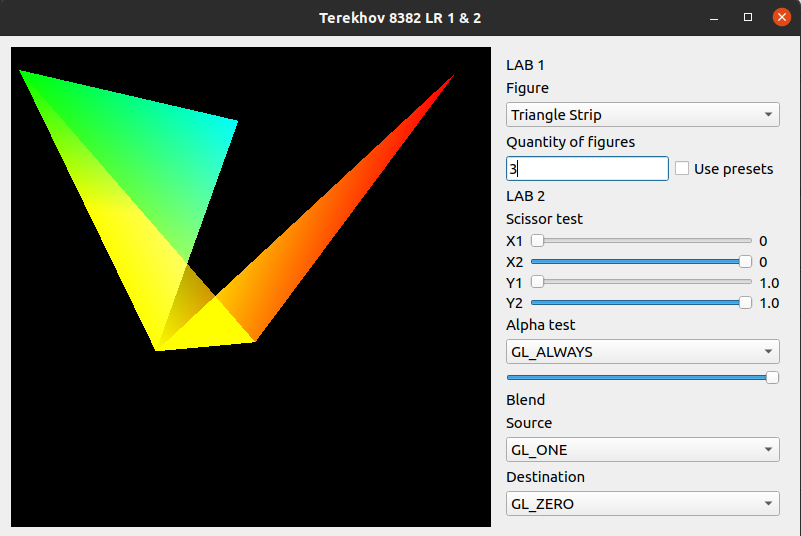
\includegraphics[width=10cm]{8}
    \caption{Примитив GL\_TRIANGLE\_STRIP}
    \label{fig:8}
\end{figure}
\begin{figure}[H]
    \centering
    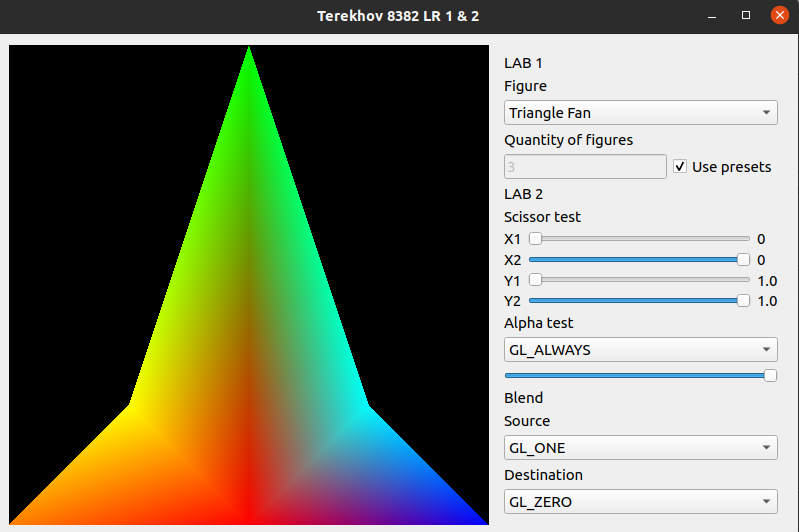
\includegraphics[width=10cm]{9}
    \caption{Примитив GL\_TRIANGLE\_FAN}
    \label{fig:9}
\end{figure}
\begin{figure}[H]
    \centering
    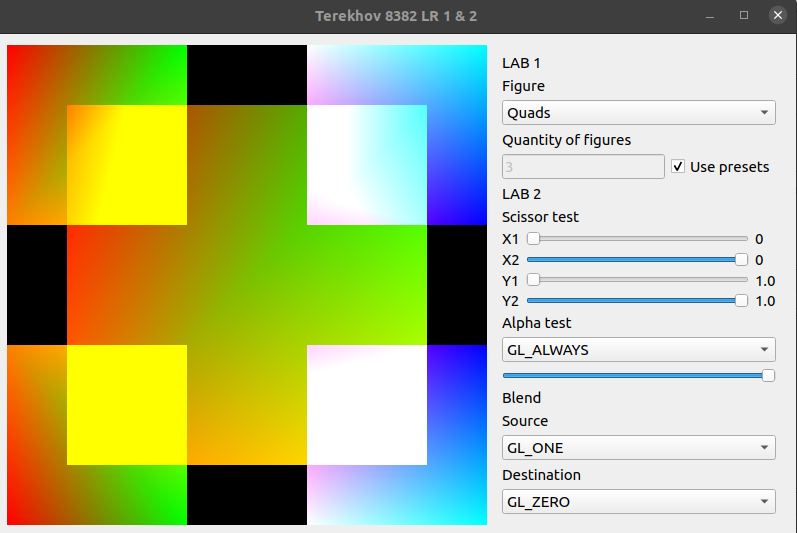
\includegraphics[width=10cm]{10}
    \caption{Примитив GL\_QUADS}
    \label{fig:10}
\end{figure}
\begin{figure}[H]
    \centering
    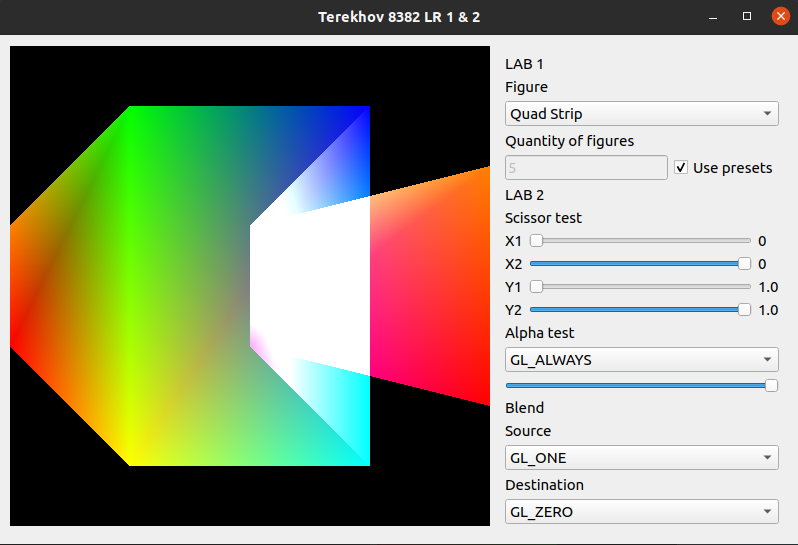
\includegraphics[width=10cm]{11}
    \caption{Примитив GL\_QUAD\_STRIP}
    \label{fig:11}
\end{figure}
\begin{figure}[H]
    \centering
    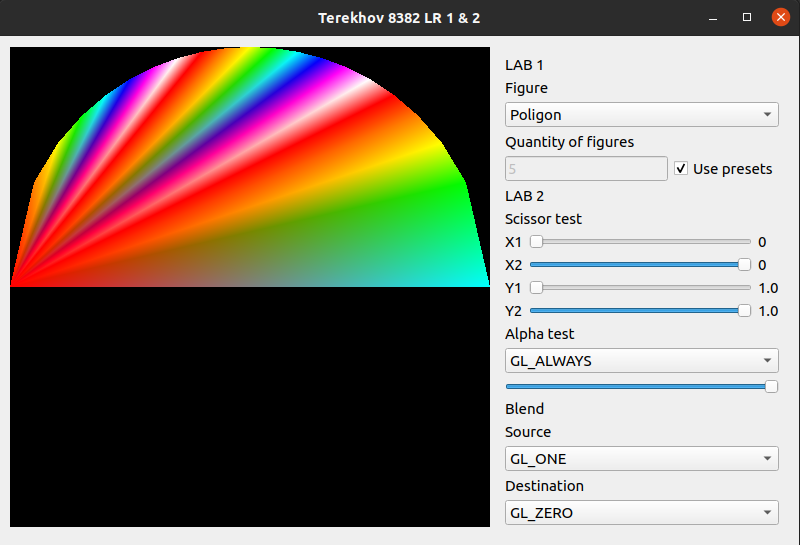
\includegraphics[width=10cm]{12}
    \caption{Примитив GL\_POLYGON}
    \label{fig:12}
\end{figure}
\section*{Вывод}
В ходе лабораторной работы была написана программа, реализующая представление определенного набора примитивов из имеющихся в библиотеке OpenGl.
Программа работает корректно.
При выполнении работы были приобретены навыки работы с графической библиотекой OpenGL.